% Options for packages loaded elsewhere
\PassOptionsToPackage{unicode}{hyperref}
\PassOptionsToPackage{hyphens}{url}
%
\documentclass[
  9pt,
  ignorenonframetext,
]{beamer}
\usepackage{pgfpages}
\setbeamertemplate{caption}[numbered]
\setbeamertemplate{caption label separator}{: }
\setbeamercolor{caption name}{fg=normal text.fg}
\beamertemplatenavigationsymbolsempty
% Prevent slide breaks in the middle of a paragraph
\widowpenalties 1 10000
\raggedbottom
\setbeamertemplate{part page}{
  \centering
  \begin{beamercolorbox}[sep=16pt,center]{part title}
    \usebeamerfont{part title}\insertpart\par
  \end{beamercolorbox}
}
\setbeamertemplate{section page}{
  \centering
  \begin{beamercolorbox}[sep=12pt,center]{part title}
    \usebeamerfont{section title}\insertsection\par
  \end{beamercolorbox}
}
\setbeamertemplate{subsection page}{
  \centering
  \begin{beamercolorbox}[sep=8pt,center]{part title}
    \usebeamerfont{subsection title}\insertsubsection\par
  \end{beamercolorbox}
}
\AtBeginPart{
  \frame{\partpage}
}
\AtBeginSection{
  \ifbibliography
  \else
    \frame{\sectionpage}
  \fi
}
\AtBeginSubsection{
  \frame{\subsectionpage}
}
\usepackage{lmodern}
\usepackage{amsmath}
\usepackage{ifxetex,ifluatex}
\ifnum 0\ifxetex 1\fi\ifluatex 1\fi=0 % if pdftex
  \usepackage[T1]{fontenc}
  \usepackage[utf8]{inputenc}
  \usepackage{textcomp} % provide euro and other symbols
  \usepackage{amssymb}
\else % if luatex or xetex
  \usepackage{unicode-math}
  \defaultfontfeatures{Scale=MatchLowercase}
  \defaultfontfeatures[\rmfamily]{Ligatures=TeX,Scale=1}
\fi
\usetheme[]{Goettingen}
\usecolortheme{rose}
% Use upquote if available, for straight quotes in verbatim environments
\IfFileExists{upquote.sty}{\usepackage{upquote}}{}
\IfFileExists{microtype.sty}{% use microtype if available
  \usepackage[]{microtype}
  \UseMicrotypeSet[protrusion]{basicmath} % disable protrusion for tt fonts
}{}
\makeatletter
\@ifundefined{KOMAClassName}{% if non-KOMA class
  \IfFileExists{parskip.sty}{%
    \usepackage{parskip}
  }{% else
    \setlength{\parindent}{0pt}
    \setlength{\parskip}{6pt plus 2pt minus 1pt}}
}{% if KOMA class
  \KOMAoptions{parskip=half}}
\makeatother
\usepackage{xcolor}
\IfFileExists{xurl.sty}{\usepackage{xurl}}{} % add URL line breaks if available
\IfFileExists{bookmark.sty}{\usepackage{bookmark}}{\usepackage{hyperref}}
\hypersetup{
  pdftitle={BIOS6643 Longitudinal},
  pdfauthor={EJC},
  hidelinks,
  pdfcreator={LaTeX via pandoc}}
\urlstyle{same} % disable monospaced font for URLs
\newif\ifbibliography
\setlength{\emergencystretch}{3em} % prevent overfull lines
\providecommand{\tightlist}{%
  \setlength{\itemsep}{0pt}\setlength{\parskip}{0pt}}
\setcounter{secnumdepth}{-\maxdimen} % remove section numbering
\AtBeginSubsection{}
\AtBeginSection{}
\ifluatex
  \usepackage{selnolig}  % disable illegal ligatures
\fi

\title{BIOS6643 Longitudinal}
\subtitle{L7 Random effect}
\author{EJC}
\date{}
\institute{Department of Biostatistics \& Informatics}

\begin{document}
\frame{\titlepage}

\begin{frame}[allowframebreaks]
  \tableofcontents[hideallsubsections]
\end{frame}
\hypertarget{random-effect}{%
\section{Random effect}\label{random-effect}}

\begin{frame}{Topics for today:}
\protect\hypertarget{topics-for-today}{}
\begin{itemize}
\item
  Inference for random effects in an LMM
\item
  Modeling random effects in an LMM, with data
\item
  Tests for variance components (brief)
\end{itemize}

\vspace{\baselineskip}

\textbf{Associated reading:}

\begin{enumerate}
\item
  Sections 3.3 and 4.1 of `LMM: inference' course notes)
\item
  Verbeke (with a focus on Ch. 7)
\item
  Hedeker (Chapters 4-7)
\end{enumerate}
\end{frame}

\hypertarget{estimation}{%
\section{Estimation}\label{estimation}}

\begin{frame}{Estimation and tests for random effects (\(\pmb b\))}
\protect\hypertarget{estimation-and-tests-for-random-effects-pmb-b}{}
\begin{itemize}
\item
  Although we can use ML or REML to estimate variance components, we may
  be interested in subject-specific random effect estimates.

  \begin{itemize}
  \item
    In particular, they may allow us to determine if there are subjects
    with unusual trends relative to the rest of the group.
  \item
    These subject-specific estimates cannot be derived from the marginal
    model.
  \item
    A common approach is to use empirical Bayes (EB) estimators. EB
    estimators have an intuitive appeal since estimates are obtained
    essentially by taking a weighted average of personal and group-level
    data.
  \end{itemize}
\end{itemize}
\end{frame}

\begin{frame}{}
\protect\hypertarget{section}{}
\begin{block}{Example 1: batting averages of Major League Baseball
players.}
\protect\hypertarget{example-1-batting-averages-of-major-league-baseball-players.}{}
\begin{itemize}
\item
  At the beginning of the season, averages tend to vary more wildly
  (between 0.000 and 1.000).
\item
  As more games are played, the averages tend to settle into range
  between 0.200 and 0.350.
\item
  An EB estimate for a particular player near the beginning of the
  season may use a higher weight for the `all-player' average and a
  lower average for that particular player to estimate that player's
  true average; later in the season the average may be weighted more
  heavily towards that player's particular average.
\end{itemize}
\end{block}
\end{frame}

\begin{frame}{}
\protect\hypertarget{section-1}{}
\begin{block}{Example 2: prevalence of a disease or illness for
individual counties in a state.}
\protect\hypertarget{example-2-prevalence-of-a-disease-or-illness-for-individual-counties-in-a-state.}{}
\begin{itemize}
\item
  Ideally, the best estimate of prevalence in a county would involve
  just the county data.
\item
  However, if collected data is sparse, then it might help to also base
  the estimate on state data as well.
\item
  The higher the variability in county data, the more the estimate is
  based on the state data, while the lower the variability in the county
  data, the more it is based on county data.
\end{itemize}
\end{block}
\end{frame}

\begin{frame}{Empirical Bayes (EB) estimators for random effects}
\protect\hypertarget{empirical-bayes-eb-estimators-for-random-effects}{}
In the Bayesian literature, the marginal distribution of \(\pmb b\) is
called the prior distribution of the parameters \(\pmb b\) since it does
not depend on the data \(\pmb Y\). Once observed values of \(\pmb Y\)
are obtained (\(\pmb y\)), the posterior distribution of b, which is
\(f(\pmb b|\pmb y)\), can be calculated. Considering \(\pmb b_i\) and
\(\pmb Y_i\) as the random effects and outcome data for individual
\(i\), the posterior distribution is:

\[
f(b_i|\pmb {Y_i = y_i}) = \frac {f(\pmb y_i |b_i)f(b_i))} {\int f(\pmb y_i|b_i) f(b_i) db_i}
\]

In the expression above, the dependence of the density function on
certain components of \(\pmb \theta\) is suppressed for notational
convenience. The mean of this posterior distribution is a Bayes
estimator of \(\pmb b_i\):

\[
\pmb {\hat b_i} (\pmb \theta) = E(b_i |\pmb Y_i = \pmb y_i)
=\int \pmb b_i f(\pmb b_i | \pmb y_i)d \pmb b_i 
= \pmb {G Z_i^{\top} V_i^{-1} (\alpha)} (\pmb {y}_i - \pmb {X}_i \pmb \beta) \ \ \ \ (6)
\]
\end{frame}

\begin{frame}{}
\protect\hypertarget{section-2}{}
The EB estimator is then computed by replacing unknown parameters
\(\pmb \alpha\) and \(\pmb \beta\) with their ML or REML estimates (and
hence the word `empirical').

We'll let \(\pmb b_i (\pmb {\hat \theta})= \pmb {\hat b_i}\) denote the
Empirical Bayes estimator. For more detail, see \textbf{section 7.2 in
Verbeke}. In terms of final notation, \(\pmb b\) and \(\pmb Y\)
represent the vector of random effects and data, respectively, for the
complete data, where data for subjects are stacked, while \(\pmb b_i\)
and \(\pmb Y_i\) are the data for individual \(i\).
\end{frame}

\begin{frame}{The EB estimators and shrinkage}
\protect\hypertarget{the-eb-estimators-and-shrinkage}{}
Predicted values based on EB estimators for \(\pmb b_i\) are a weighted
average of subject-specific data and group-averaged data, giving it an
intuitive appeal:

\[
\pmb {\hat Y_i} = \pmb {X_i  \hat \beta} + \pmb {Z_i b_i}   = \pmb X_i \pmb {\hat \beta} + \pmb {Z_i GZ_i^{\top}V_i}^{-1} (\pmb {Y_i-X_i \beta})    
\]

\vspace{-5mm}

\[
= (\pmb I_{r_i}- \pmb {Z_i GZ_i^{\top} V_i^{-1}}) \pmb {X_i  \beta} + \pmb {Z_i GZ_i^{\top}V_i^{-1} Y_i} = \pmb {R_i V_i^{-1} X_i  \hat \beta} + (\pmb I_{r_i} - \pmb {R_i V_i}^{-1}) \pmb Y_i
\]

\((\pmb I_{r_i} - \pmb {R_i V_i}^{-1})\) is a weighted average of the
estimated population average profile and the observed data.

This demonstrates that \(\pmb {\hat Y_i}\) are shrunk towards the mean
(relative to \(\pmb Y_i\)).
\end{frame}

\begin{frame}{}
\protect\hypertarget{section-3}{}
When residual variability (modeled through \(\pmb R_i\)) is large in
relation to between-subject variability (accounted for in
\(\pmb V_i^{-1}\)), the population-averaged profile
(\(\pmb {X_i \beta}\)) will have more weight, which makes sense since
there is less certainty about individual data. (You can think of
\(\pmb R_i\) as the ``numerator'' and \(\pmb V_i\) as the
``denominator'' in the quantity \(\pmb {R_i V_i}^{-1}\).)

Alternatively, when residual (within-subject) variability tends to be
smaller and between-subject variability greater, then \(\pmb Y_i\) will
have more weight.

The EB estimators themselves exhibit the shrinkage property:
\(Var[\pmb {Lb}_i] \leq Var[\pmb {L\hat b}_i]\) for any \(1 \times q\)
real-valued vector \(\pmb L\). Remember also that \(E[\pmb b_i] = 0\).
Thus the EB estimators are shrunk towards 0. For more detail, see
\textbf{Verbeke}.
\end{frame}

\begin{frame}{Inference associated with EB estimators}
\protect\hypertarget{inference-associated-with-eb-estimators}{}
The quantity \(Var[\pmb {\hat b}_i (\pmb \theta)]\) can be derived
easily by substituting the MLE in for \(\pmb \beta\) and noting that it
is a linear form of \(\pmb y_i\). (Laird and Ware, 1982, consider the
Bayes estimator as in (6), but with \(\pmb \beta\) replaced with its
MLE; they then derive theoretical results when covariance parameters are
known or unknown.) The result is:

\[
Var[\pmb {\hat b}_i (\pmb \theta)] = \pmb {G_i Z^{\top}_i\Big(V_i^{-1}-V_i^{-1} X_i (\sum X_i^{\top}V_i^{-1} X_i)^{-1} X_i^{\top}V_i^{-1}\Big)Z_i G_i}
\]

\begin{itemize}
\item
  \(Var[\pmb {\hat b}_i (\pmb \theta)]\) is not the same as
  \(Var[\pmb b_i |\pmb Y_i= \pmb y_i]\); it is
  \(Var \Big[ E[\pmb b_i (\pmb \theta)|\pmb y_i]\Big]\).
\item
  For inference, \(Var[\pmb {\hat b}_i (\pmb \theta) - \pmb b_i]\) is
  used rather than \(Var[\pmb {\hat b}_i (\pmb \theta)]\) because the
  former take into account the variability in \(\pmb b_i\). This
  quantity is:
  \(Var[ \pmb {\hat b}_i (\pmb \theta)- \pmb b_i] = \pmb G_i - Var[ \pmb {\hat b}_i (\pmb \theta)] = \pmb G_i - \pmb {G_i Z_i^{\top}\Big({V_i^{-1}-V_i^{-1} X_i (\sum X_i^{\top}V_i^{-1} X_i)^{-1} X_i^{\top}V_i^{-1}}\Big)Z_i G_i}\)
\end{itemize}

In order to estimate \(Var[ \pmb {\hat b}_i (\pmb \theta)- \pmb b_i]\)
we typically just `plug in' numerical values for unknown
\(\pmb \theta\), not accounting for the added variability due to use of
estimated values. In light of this, the selection of DF can help control
the accuracy of inferential results for random effects, similar to that
described previously for inference of fixed effects.
\end{frame}

\begin{frame}{}
\protect\hypertarget{section-4}{}
\(t\)-tests can be constructed for random effects using relevant
approximate \(t\) quantities.

\begin{itemize}
\item
  For example, if \(\pmb b_i\) contains just a random intercept (i.e.,
  \(\pmb b_i= b_{0i}\)) then we can use
  \(t = \frac {(\hat b_{0i} - b_{0i}) - E[\hat b_{0i} - b_{0i}]} {\widehat {SE} (\hat b_{0i} - b_{0i})}\),
  which reduces to
  \(t=\frac {{\hat b}_{0i}} {\widehat {SE} (\hat b_{0i} - b_{0i})}\)
  under the null, for the test of \(H_0: b_{0i}=0\).
\item
  For models with multiple random effect terms, we can carry out
  \(t\)-tests separately for each component of \(\pmb b_i\) (and
  subject). As before, the DF (\(\nu\)) is ideally chosen to get the
  correct distribution of the test statistic under \(H_0\); available
  methods to do this are as previously described.
\item
  Theory also exists for tests \(H_0: \pmb {Lb} = 0\) versus
  \(H_1: \pmb {Lb} \neq 0\). However, in practice, I have not yet found
  the need to use this.
\item
  A \(100 \times (1 – \alpha) \%\) confidence interval for an element
  \(b_{hi}\) of \(b_i\), is
  \(\hat b_{hi} \pm t_{\nu,\ \frac \alpha 2} \times \widehat {SE} (\hat b_{hi} - b_{hi})\).
\end{itemize}
\end{frame}

\begin{frame}{}
\protect\hypertarget{section-5}{}
In SAS, when you request a solution for the random effects, the
`Estimate' will be numerical versions of (6), while `Std Err Pred' is
the square root of (diagonal elements of)
\(Var[ \pmb {\hat b}_i (\pmb \theta) - \pmb b_i]\). The calculated
variance of the random effect estimates (using the `population' version)
will be the same as \(\widehat {Var} [\pmb {\hat b}_i (\pmb \theta)]\)
(here, the hat on `Var' indicates that estimated values of
\(\pmb \theta\) are `plugged into' the calculation) and will be somewhat
less than \(\sigma_b^2\), reflecting the shrinking of the estimates back
to the estimated population mean.
\end{frame}

\begin{frame}{Computation of estimates and associated variances for
random effects}
\protect\hypertarget{computation-of-estimates-and-associated-variances-for-random-effects}{}
\textbf{see course notes}
\end{frame}

\begin{frame}{Empirical Bayes estimators for LMMs with random
intercepts}
\protect\hypertarget{empirical-bayes-estimators-for-lmms-with-random-intercepts}{}
We have discussed Empirical Bayes estimators of random effects in mixed
models. They have an intuitive appeal because they can be expressed as
weighted averages of subject-specific information and population-average
information.

\begin{itemize}
\item
  The greater the variability of the subject data, the higher the weight
  is placed on the population average;
\item
  The more consistent the subject data is, the higher the weight is
  placed on the subject portion.
\item
  In previous notes, the weighted average was expressed for predicted
  values (\(\hat Y_i\)) from an LMM.
\item
  It was briefly mentioned that the random effects estimates themselves
  (\(\pmb {\hat b}_i\)) are shrunk towards the population mean (relative
  to \(\pmb b_i\)), such that
  \(Var[ \pmb {\hat b}_i ] \leq Var[\pmb b_i]\).
\item
  The amount of shrinkage depends on residual variance relative to
  subject variance. To study this further, we'll consider LMMs with
  random intercept terms.
\end{itemize}
\end{frame}

\begin{frame}{}
\protect\hypertarget{section-6}{}
It was mentioned that the random effects estimates (\(\pmb {\hat b}_i\))
are shrunk towards the population mean (relative to \(\pmb b_i\)), such
that \(Var[\pmb L \pmb {\hat b}_i] \leq Var[\pmb {Lb}_i ]\) for a
\(1 \times q\) real-valued vector \(\pmb L\).

\begin{itemize}
\item
  A special case of this is \(Var[{\hat b}_{hi}] \leq Var[b_{hi}]\), for
  \(h = 1,\ ...\ ,\ q\). This is easy to prove, since
  \(Var[ \pmb {\hat b}_i - \pmb b_i] + Var[\pmb {\hat b}_i] = \pmb G_i\)
  , and the diagonal elements must be nonnegative.
\item
  The only time equality holds, such that
  \(Var[\pmb {\hat b}_{hi}] = Var[b_{hi}]\), is when
  \(Var[\pmb {\hat b}_{hi} - \pmb b_{hi}]=0\). The amount of shrinkage
  in estimators depends on residual variance relative to subject
  variance. To study this further, we'll consider LMMs with random
  intercept terms.
\end{itemize}
\end{frame}

\begin{frame}{}
\protect\hypertarget{section-7}{}
If the only random term in the model is an intercept term (for subjects)
and \(\pmb R_i=\sigma^2 \pmb I\), (6) will reduce, since \(\pmb G\) only
has one element (the variance of the random intercepts, call it
\(\sigma_b^2\)), and \(\pmb Z_i^{\top}\) is a row vector of 1's, call it
\(\pmb J_{(1\times r)}\). For this case:

\[
\pmb V_i^{-1}=(\sigma_b^2 \pmb J_{(r_i\times r_i )}-\sigma_\epsilon^2 \pmb I_{(r_i\times r_i )} )^{-1}=
\frac 1 {\sigma _\epsilon^2} {\Big(\pmb I_{(r_i\times r_i )} - \frac {(\sigma_b^2)}{ (\sigma_\epsilon^2+r_i \sigma_b^2 )} \pmb J_{(r_i\times r_i )} \Big)}  
\]

Ultimately, the Bayes estimator reduces to:

\[ 
{\hat b}_i (\pmb \theta) = \lambda \Big(\bar Y_i - \frac {\sum_j \pmb X_{ij}^r \pmb \beta} {r_i}\Big) \ \ \ \ (7)
\]

\begin{itemize}
\tightlist
\item
  where \({\bar Y_i}\) is the mean response for subject \(i\),
  \(\pmb X_{ij}^r\) is the \(j\)th row of \(\pmb X_i\), and
  \(\lambda=\frac {r_i \sigma_b^2} {\sigma_\epsilon^2+r_i \sigma_b^2}\).
\end{itemize}

Note that \(\lambda\) is between 0 and 1; it is the weight used in the
averaging of subject-specific and population average statistics. (Note
also that \(u\) \alert {there is no u, and I have no idea} is unbolded
since it involves just one estimator.) Greater between-subject
variability relative to within-subject variability will yield larger
values of \(\lambda\) (just like the ICC), but so will increasing the
number of repeated measures.
\end{frame}

\begin{frame}{}
\protect\hypertarget{section-8}{}
For practice, show that (7) holds, starting with (6). (You can use the
given result for \(\pmb V_i^{-1}\).) When there is only a random
intercept term and fixed intercept in the model {[} \$Y\_\{ij\} =
\beta\emph{0 + b\_i + \epsilon}\{ij\} \$;
\(b_i \stackrel {iid} \sim \mathcal N(0,\ \sigma_b^2)\), independently
of
\(\epsilon_{ij} \stackrel {iid} \sim \mathcal N (0,\ \sigma_{\epsilon}^2)\);
call it the `simple random intercept model'{]}, (7) becomes
\(\pmb {\hat b}_i (\pmb \theta)=\lambda[\bar Y_i- \beta_0]\ \ \ \ \ (8)\)

We can consider \(\lambda\) as the shrinkage factor. What is being
shrunk is the difference between the estimate of the random intercept
for subject \(i\) and the population mean. If we add the population
mean, \(\beta_0\), we get the estimate for subject \(i\) in context of
the population:

\[
\lambda(\bar Y_i- \beta_0)+ \beta_0 = \lambda\bar Y_i+(1-\lambda) \beta_0\ \ \ \ \ (9)
\] which is a weighted average of \(\pmb {\bar Y}_i\) and \(\beta_0\).

In practice we typically replace unknown parameters \(\lambda\) (which
involves \(\sigma_b^2\) and \(\sigma_\epsilon^2\)) and \(\beta_0\) in
(8) and (9) with their estimators, yielding EB estimators.

For the simple random intercept model, the variance of the Bayes
estimator is

\[
Var[{\hat b}_i (\pmb \theta)]= \frac {n-1} n  \lambda \sigma_b^2\ \ \ \ \ (10)
\]
\end{frame}

\begin{frame}{Verify for practice.}
\protect\hypertarget{verify-for-practice.}{}
As noted earlier, the variance quantity normally used in inference to
account for randomness in \(\pmb b_i\) is:

\[
Var[{\hat b}_i (\pmb \theta)-b_i]=\sigma_b^2 - Var[{\hat b}_i (\pmb \theta)] 
=\sigma_b^2 - \frac {n-1} n \lambda \sigma_b^2  = \frac {\big(1-\lambda (n-1)\big)} n   \sigma_b^2 \ \ \ \ (11)
\]

Since the variance of EB estimators is more difficult to tackle, we
usually work with the variance quantities of the Bayes estimators, in
(10) and (11). But in practice we do then typically plug in values of
unknown variances in the quantity, which I will denote as
\(\widehat Var[{\hat b}_i (\pmb \theta)]\) and
\(\widehat Var[{\hat b}_i (\pmb \theta)-b_i]\).

For the random intercept model we know that
\(Var[{\hat b}_i (\pmb \theta)-b_i] + Var[{\hat b}_i (\pmb \theta)]=\sigma_b^2\)
(more generally, that
\(Var[ \pmb {\hat b}_i (\pmb \theta)-b_i]+Var[ \pmb {\hat b}_i (\pmb \theta)]=\pmb G_i\)).
For fixed variances, we know that \(\lambda \rightarrow 1\) as the
number of repeated measures, \(r_i\) is increased (and also n), in which
case \(Var[{\hat b}_i (\pmb \theta)] \rightarrow \sigma_b^2\), and hence
\(Var[{\hat b}_i (\pmb \theta)-b_i]\rightarrow0\).
\end{frame}

\hypertarget{the-mt.-kilimanjaro-data}{%
\section{The Mt. Kilimanjaro data}\label{the-mt.-kilimanjaro-data}}

\begin{frame}{The Mt. Kilimanjar}
\protect\hypertarget{the-mt.-kilimanjar}{}
\begin{itemize}
\item
  Oxygen saturation, or SAO2, can be measured as the percentage of
  hemoglobin molecules which are oxgenated (oxyhemoglobin) in arterial
  blood.
\item
  The normal range is \(> 95\%\), however at higher altitudes this
  percentage tends to go down.
\item
  This measure was taken on hundreds of subjects that climbed Mt.
  Kilimanjaro (the tallest mountain on the continent of Africa).
\item
  The following graph shows SAO2 versus altitude, along with a quadratic
  fit using a linear mixed model.
\item
  The bubble plot was used because many values occurred on the same
  \((x,\ y)\) location; bubbles indicate how many subjects occurred at
  each point, the bigger the bubble, the more subjects at that location.
\end{itemize}
\end{frame}

\begin{frame}{}
\protect\hypertarget{section-9}{}
\begin{itemize}
\item
  Although these are repeated measures data, lines connect points are
  suppressed due to the large amount of data.
\item
  Superimposed on the bubble plot are two curves, one showing subjects
  that were taking a medication to help prevent symptoms of
  high-altitude sickness (blue), and those that were not (not).
\item
  Those taking the medication are able to maintain slightly higher
  oxygen levels (which may also help reduce symptoms of high altitude
  sickness), with greater differences at higher altitudes.
\item
  These differences are statistically significant after about 3km, but
  it may be somewhat subjective as to whether the small differences as
  worth taking the medication.
\end{itemize}
\end{frame}

\begin{frame}{}
\protect\hypertarget{section-10}{}
\begin{center}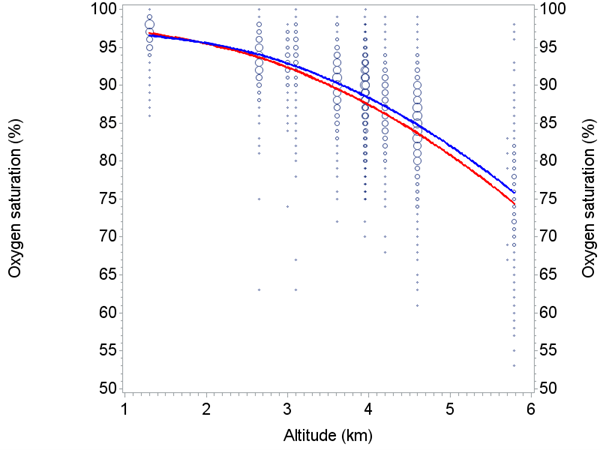
\includegraphics[width=0.6\linewidth]{figs_L7/f1} \end{center}

The bubble plot was generated by using the `bubble' statement in PROC
GPLOT. I then overlayed the fitted curves from the fitted linear mixed
model in a subsequent `plot2' statement.
\end{frame}

\begin{frame}{}
\protect\hypertarget{section-11}{}
Below is the SAS code used to fit the mixed model:

\begin{center}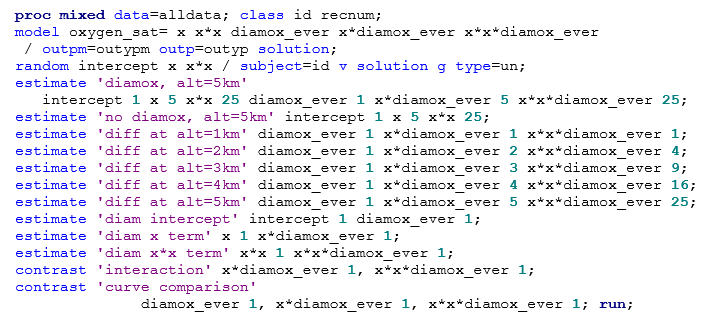
\includegraphics[width=0.6\linewidth]{figs_L7/f2} \end{center}
\end{frame}

\begin{frame}{Abbreviated output:}
\protect\hypertarget{abbreviated-output}{}
\begin{center}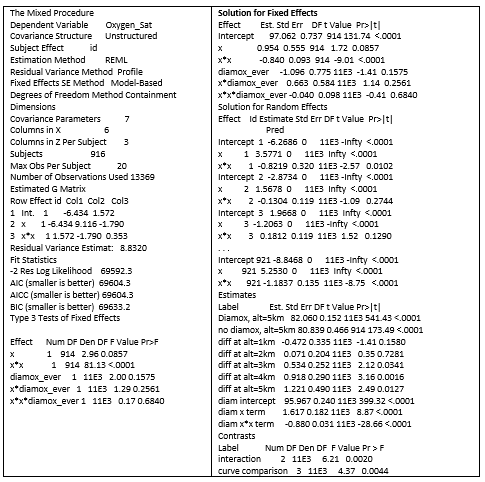
\includegraphics[width=0.6\linewidth]{figs_L7/f3} \end{center}
\end{frame}

\begin{frame}{Some interesting things to point out from the output:}
\protect\hypertarget{some-interesting-things-to-point-out-from-the-output}{}
The variance of the intercept was estimated to be 0. However, no penalty
was added for this in the AIC; essentially, that parameter is removed
from the model. You can tell this is the case because the difference
between \(-2 log\ (Restriced\ Likelihood)\) and the AIC is 12, so 6
parameters are accounted for (5 in \(\pmb G\) matrix, plus residual
variance).

Notice also that subject estimates of intercept and some linear terms
have predicted standard errors of 0; our interpretation should be that
these standard errors could not be estimated, rather than that they were
true 0's.

Estimates included demonstrate that although differences between
medication users and non-users appeared to be minor, visually, they were
statistically significant, with greater significance at higher
elevations.

The contrasts indicate that there were differences between curves that
could not be accounted for by intercept differences alone (see
`interaction' test, \(p=0.0020\)), and that the curves were not the same
(including both `interaction' and y-intercept differences,
\(p=0.0044\)).
\end{frame}

\begin{frame}{}
\protect\hypertarget{section-12}{}
\begin{center}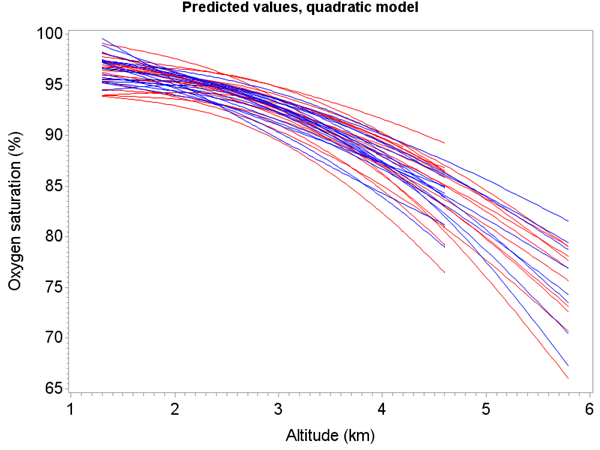
\includegraphics[width=0.6\linewidth]{figs_L7/f4} \end{center}

The graph above shows predicted values for subjects, from the mixed
model, using only 20 per group (no medication -- red / medication --
blue) are plotted. Differences for subjects are due to the use of the
intercept, linear and quadratic random effect terms. Notice that the
predicted curves tend to fan out at higher altitudes, just like the raw
data.
\end{frame}

\begin{frame}{}
\protect\hypertarget{section-13}{}
\begin{center}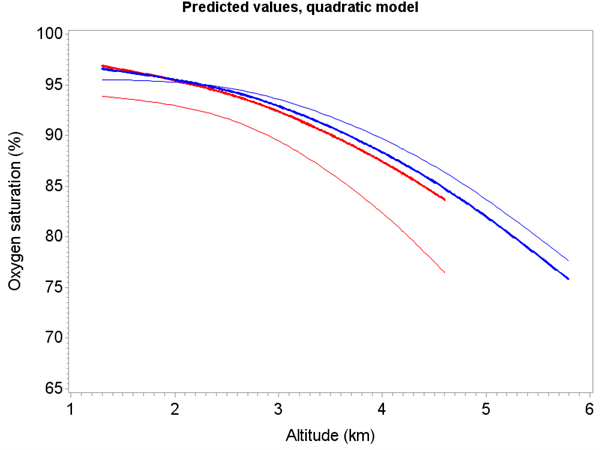
\includegraphics[width=0.6\linewidth]{figs_L7/f5} \end{center}

This graph shows population-averaged estimates (thick red and blue) and
two subject curves (thin red and blue: see subject ID's 1 (red) and 2
(blue) on previous SAS output.

Recall that random effect estimates are deviations from fixed effect
estimates. Notice how the red subject curve has much greater curvature
than the thick red curve, compared with the thin and thick blue lines.
This is echoed in the tests on the previous output, where the
\(t\)-tests indicate that subject 1 has significant difference in
quadratic effect compared with its population counterpart
(\(p=0.0102\)), while the blue does not (\(0.2744\)).

Both subject curves have lower intercepts and higher coefficients for
the first order term, although we are unable to conduct tests to see if
they are significantly different than population counterparts, since SEs
could not be determined. Accounting for serial correlation in the data
improves the fit even more. This will be discussed more in the following
sections.
\end{frame}

\hypertarget{tests-for-variance-components}{%
\section{Tests for variance
components}\label{tests-for-variance-components}}

\begin{frame}{Tests for variance components}
\protect\hypertarget{tests-for-variance-components-1}{}
We can use `COVTEST' as an option in the PROC MIXED statement for tests
involving covariance parameters, using Wald \(Z\) tests.

We can also test for a `significant additions' of random terms to a
model (e.g., when including the random slope to an LMM with a random
intercept) using likelihood ratio test methods. Here we compare changes
in \(–2ln(\mathcal L)\) between models, which has an asymptotic
\(\chi^2\) distribution with DF = difference in the number of covariance
parameters between the 2 models.

For both approaches, tests are more valid when certain regularity
conditions hold. See \textbf{Verbeke, pages 64-66} for more detail.
\end{frame}

\hypertarget{summary}{%
\section{Summary}\label{summary}}

\begin{frame}{Summary}
\protect\hypertarget{summary-1}{}
\end{frame}

\end{document}
